 \leadauthor{Daniel Anderson}

\title{Gene-space \textit{de Bruijn} graphs enable accurate detection of multi-copy antimicrobial resistance genes directly from long read sequencing data}
\shorttitle{}

\author[1, \Letter]{Daniel Anderson \orcidlink{0000-0003-4422-9520}}
\author[1]{Leandro Lima \orcidlink {0000-0001-8976-2762}}
\author[2]{Trieu Le \orcidlink {0009-0000-2555-0496}}
\author[3]{Louise M. Judd \orcidlink {0000-0003-3613-4839}}
\author[3]{Ryan R. Wick \orcidlink {0000-0001-8349-0778}}
\author[1,2]{Zamin Iqbal \orcidlink {0000-0001-8466-7547}}

\affil[1]{European Bioinformatics Institute, Hinxton, Cambridge CB10 1SD, UK}
\affil[2]{Milner Centre for Evolution, University of Bath, UK}
\affil[3]{Department of Microbiology and Immunology, The University of Melbourne at the Peter Doherty Institute for Infection and Immunity, Melbourne, Victoria, Australia}
\date{}

\maketitle

\begin{abstract}
Abstract of the paper goes here.
\end{abstract}

\begin{keywords}
keyword1 | keyword2 | keyword3
\end{keywords}

\begin{corrauthor}
dander\at ebi.ac.uk
\end{corrauthor}

\section*{Introduction}

Antimicrobial resistance (AMR) in bacteria is a significant global health challenge and a major threat to modern medical science. The development and spread of AMR is primarily driven by genetic changes that can be attributed to spontaneous mutations or to the acquisition of AMR genes from external sources \cite{10.1038/s41576-019-0108-4}. In many cases, the presence of an AMR gene or SNP is sufficient to confer resistance to a single or a broad spectrum of antimicrobials \cite{10.1128/AEM.02873-15}. However, increasing evidence has demonstrated dosage-dependent effects of AMR gene copy number variation on minimum inhibitory concentration (MIC) \cite{10.1128/aac.02026-19, 10.1128/AAC.46.10.3334-3336.2002}. Therefore, accurate identification of AMR gene content is crucial for the surveillance of AMR, and for predicting and quantifying resistance. Numerous tools have been developed to identify genes or alleles known to be associated with AMR \cite{Feldgarden2021, Bortolaia2020, 10.1093.nar.gkz935, Seemann2023, Hunt2017, Bradley2015} and these typically require sequence assembly as a prerequisite. 

Sequence assembly involves taking the unordered base called sequencing reads output from next generation sequencing technologies and attempting to generate a consensus sequence of the genome. This is usually done by constructing overlap graphs or \textit{de-Bruijn} graphs (DBGs) from \textit{k}-mers, then traversing paths through the graph to obtain the assembly <CITATION>. Many bacterial genomes are repetitive and assemblers struggle to resolve the sequences of these repeats on a fundamental level. Illumina reads, although highly accurate, are much shorter than the maximum repeat size, so reads containing sequences from large duplications cannot be properly placed in the genome \cite{KOREN2015110}. ONT reads are often longer than the size of these repeating units, but large-scale errors can occur in complex regions of the assembly graph, leading to duplications being collapsed or sequence being absent from the assembly entirely \cite{10.12688/f1000research.21782.1, 10.1186/s13059-021-02483-z, FosterNyarko2023}. This is a significant concern using AMR genotyping tools that depend on the assembly because complicated regions of the genome tend to be the result of recombination events and are enriched with epidemiologically relevant traits, leading to incorrect prediction of antibiotic susceptibility when misassembled. To overcome the limitations of requiring a perfect assembly, several approaches have been developed to genotype AMR genes directly from sequencing reads \cite{Bortolaia2020, Bradley2015, Hunt2017}. However, all of these improperly handle multi-copy AMR genes.

In this work we present Amira, a tool to genotype AMR genes directly from long read sequencing data. Amira uses the genomic context of AMR genes to differentiate and cluster the reads corresponding to different copies of multi-copy genes and obtain the alleles of each copy. We show that Amira achieves improvements in AMR gene detection and allele accuracy for both single and multi-copy AMR genes compared to long read-only assembly- and read-based methods. 

\section*{Results}

\subsection*{Constructing a reference pan-genome for \textit{E. coli}}

We construct a pan-genome reference from the gene annotations of 20 \textit{E coli} samples, and supplement it with 2,566 plasmid-specific genes and 7,062 acquired AMR gene reference alleles from the NCBI Bacterial Antimicrobial Resistance Reference Gene Database. Our quality control filtered 40 of these reference alleles. We then use the tool pandora to construct a pan-genome reference graph (panRG) from these multiple sequence alignments.  In total our panRG contained 98,796 alleles across 11,665 clusters of orthologous genes.

\subsection*{Amira leverages the length of long reads to differentiate multi-copy AMR genes by their genomic context}

We developed a method, implemented in a tool called Amira, for detecting multi-copy AMR genes directly from long read sequencing data. The basic idea was first to identify AMR  genes and the genes around them, on long read sequences using a reference pan-genome of genes. Second, to construct a \textit{de Bruijn} graph (DBG) in gene space and apply correction methods to the graph and the underlying reads (Fig.\ref{fig:1}a and \ref{fig:1}b). Finally, to cluster the reads pertaining to different copies of the same AMR gene by their path in the graph and independently obtain the nucleotide sequences of each copy (Fig.\ref{fig:1}c).

There are standard techniques to construct and correct DBGs in nucleotide space: \textit{k}-mers are identified by using a sliding window and adjacent \textit{k}-mers are connected by an edge. The main source of errors are sequencing errors, which are rare and can be removed by removing low frequency \textit{k}-mers. However, in this gene-space scenario, genes are detected along a read by identifying and chaining minimizer “hits” to genes that are represented by a species-specific reference pan-genome (panRG). We construct and map the reads to the panRG using Pandora and store an ordered list of gene, gene directions and gene coordinates on each read. The main source of errors in our approach is false negative or positive gene calls by Pandora. False negatives arise as a result of sequencing errors or insufficient representation of the diversity of the gene in the panRG, which we moderate by setting a minimum length of 250bp for genes and clean during gene DBG correction using node coverage thresholds. However, false positives are mostly systematic and the result of the genuine presence of fragmented forms of the called gene. We address these up front by excluding all transposase genes from our panRG, then at runtime apply a read correction method that merges paths through bubbles in the graph that originate from the same underlying nucleotide sequence. We then rebuild the graph from the corrected reads and iteratively repeat the process until there are no more corrections (see Methods for further details).

We then iterate through each unique AMR gene that has been identified by Pandora, and for each, go through a 2-step clustering process, with the aim of separating the reads containing different copies of the gene. In the first step, reads are clustered based on the immediate genomic context $(k - 1) / 2$ genes upstream or downstream of the AMR gene or a tandem array of AMR genes.  In the second step, the full length of the reads are used to infer minimum-length paths through the graph that differentiate one copy of the gene from another (see Fig.\ref{fig:1}c; further details in Methods). Each cluster then corresponds to an inferred copy of the AMR gene, and a consensus sequence is obtained using racon.

\begin{figure*}
\centering
\includegraphics[width=1\linewidth]{Figures/figure_1.pdf}
\caption{An outline of the Amira gene DBG construction (a) and correction (b) approach and read assignment (c). Red has been used to indicate the presence of AMR genes, and blue used for all other genes. a) Genes and gene directions are detected on each sequencing read using Pandora. A DBG is constructed in gene space of the gene calls, with a forward and backward edge connecting adjacent nodes. b) The gene DBG is corrected by applying an iterative correction algorithm that consists of dead end trimming and bubble popping. c) An outline of the Amira read clustering approach. Amira uses the corrected gene DBG to cluster the reads corresponding to multi-copy AMR genes based on their path through the graph, first by clustering based on the presence of internal blocks of contiguous nodes containing AMR genes, then sub-clustering using blocks upstream and downstream of the internal blocks. Red nodes contain AMR genes and orange, purple and pink are used to indicate the paths of reads through this region of the graph.}
\label{fig:1}
\end{figure*}

\subsection*{Simulations confirm that Amira resolves complex duplications of AMR genes with sufficiently long reads}

We simulated six scenarios to evaluate Amira and the effect of read depth and length on AMR gene calling accuracy by artificially inserting real AMR-gene-containing sequences of increasing complexity into a reference \textit{E. coli} chromosome and plasmid with no AMR genes. These scenarios were: a single isolated AMR gene on the chromosome, a two-copy gene with one copy on chromosome and the other on the plasmid, a tandem array of six duplicated AMR genes on the chromosome, a 54.2 kb multi-gene array on the chromosome and 36.5 kb array on the plasmid, and finally the same as the previous scenario with an additional 37.9 kb array on the chromosome \cite{TamamuraAndoh2021}. We define AMR gene recall as the proportion of true copies of a gene that were identified. Recall showed a strong positive correlation with increased read depth, and maximum accuracy was achieved at 40x and 80x depth due to there being a sufficient number of reads in the longer tail of the read length distribution (Fig.\ref{fig:2}). Gene recall was also highly correlated with read length, particularly in scenarios 4, 5 and 6, where longer reads could compensate for lower read depth.

The precise allelic identity of AMR genes correctly identified by Amira was highly accurate even at low read depths, with a mean allelic identity of 99.4\% at 5x depth, 99.7\% at 10x depth and 99.9\% at 20x, 40x and 80x depth.

\begin{figure*}
\centering
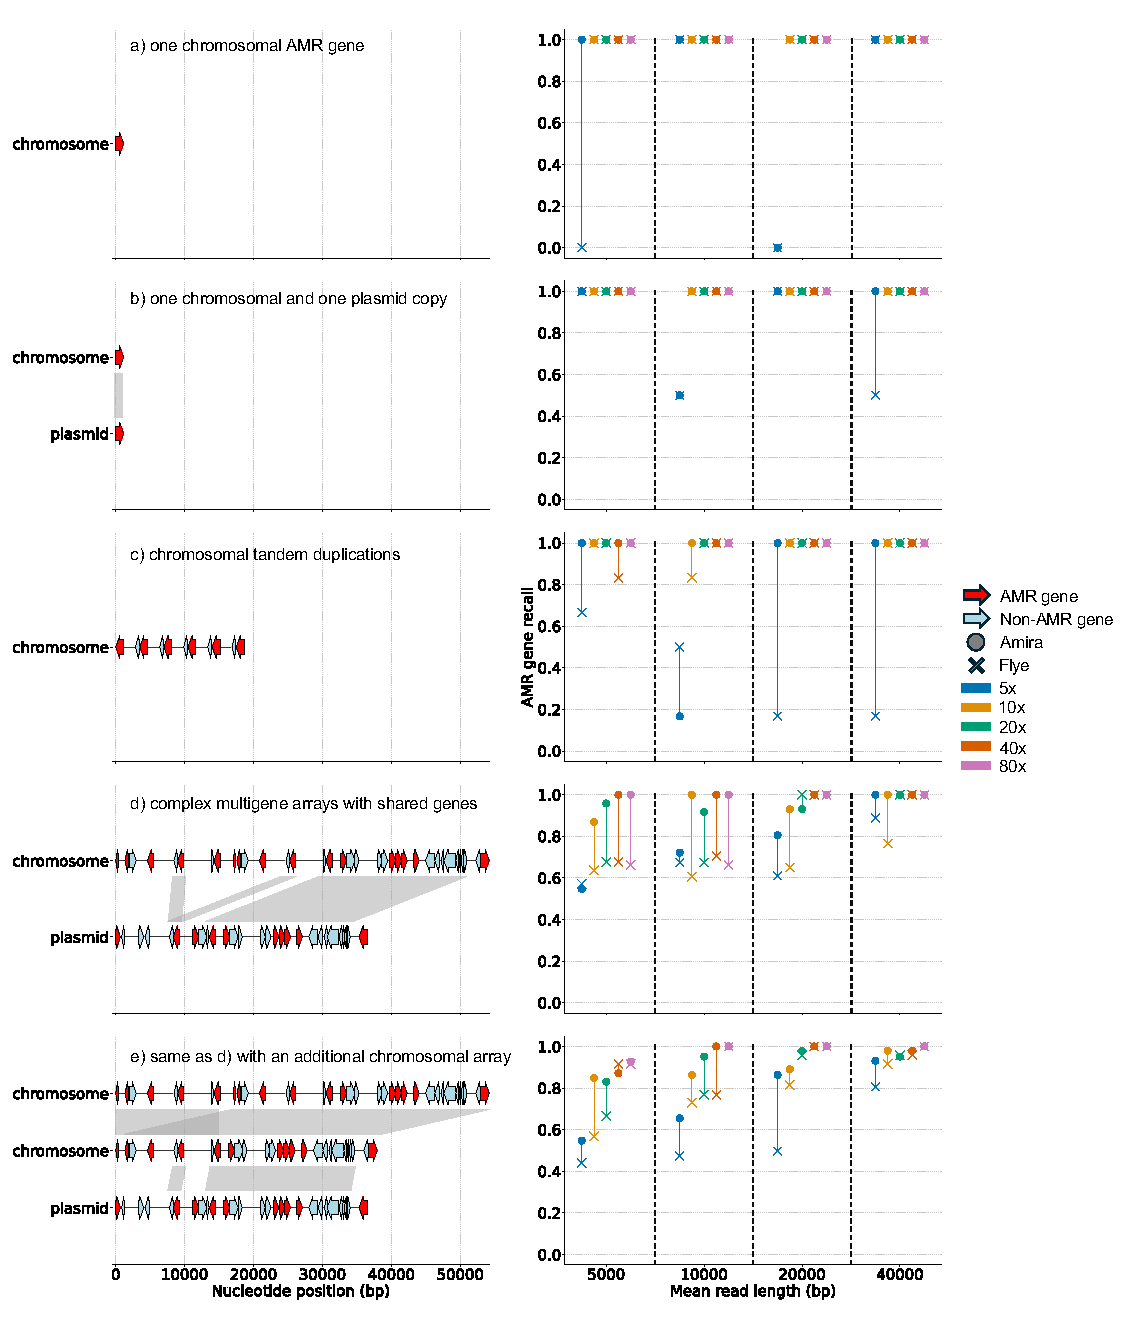
\includegraphics[width=1\linewidth]{Figures/figure_2.pdf}
\caption{Context plots detailing the AMR gene (red) and context gene (blue) content of five simulation scenarios (left) and the AMR gene recall of Amira and AMRFinderPlus applied to long reads simulated from each scenario (right). We artificially inserted each region into the chromosome or plasmid of an artificial \textit{E. coli} assembly containing no AMR genes, and applied Amira and Flye with AMRFinderPlus to the reads simulated from each simulated assembly. The x-axis of the left-hand plots shows the length of the inserted region in base pairs, and the y-axis shows which contig in the reference each region was inserted into. The x-axis of the right hand plots show the mean read simulated read lengths (5 kb, 10 kb, 20 kb and 40 kb), the y-axis the AMR gene recall. Each colour indicates the simulated read depth (5x, 10x, 20x, 40x or 80x).}
\label{fig:2}
\end{figure*}

\subsection*{Amira outperforms assembly-based AMR gene callers}

Since simulations do not fully reflect the error profiles and AMR gene complexity of real long read sequencing data, we next evaluate how Amira performs on a dataset of 32 diverse \textit{E. coli} with illumina and nanopore reads available and known AMR gene content. Ten of these samples were sequenced using R10.4 Nanopore flow cells and 22 using R9.4.1. We ensure our evaluation samples span across the \textit{E. coli} phylogeny, and use samples independent from those used to construct the reference panRG (Fig.\ref{fig:3}). Our dataset contains 18 isolates with at least one multi-copy AMR gene, with one sample containing seven copies of a \textit{blaCMY} gene, of which six are in tandem. 

\begin{figure*}
\centering
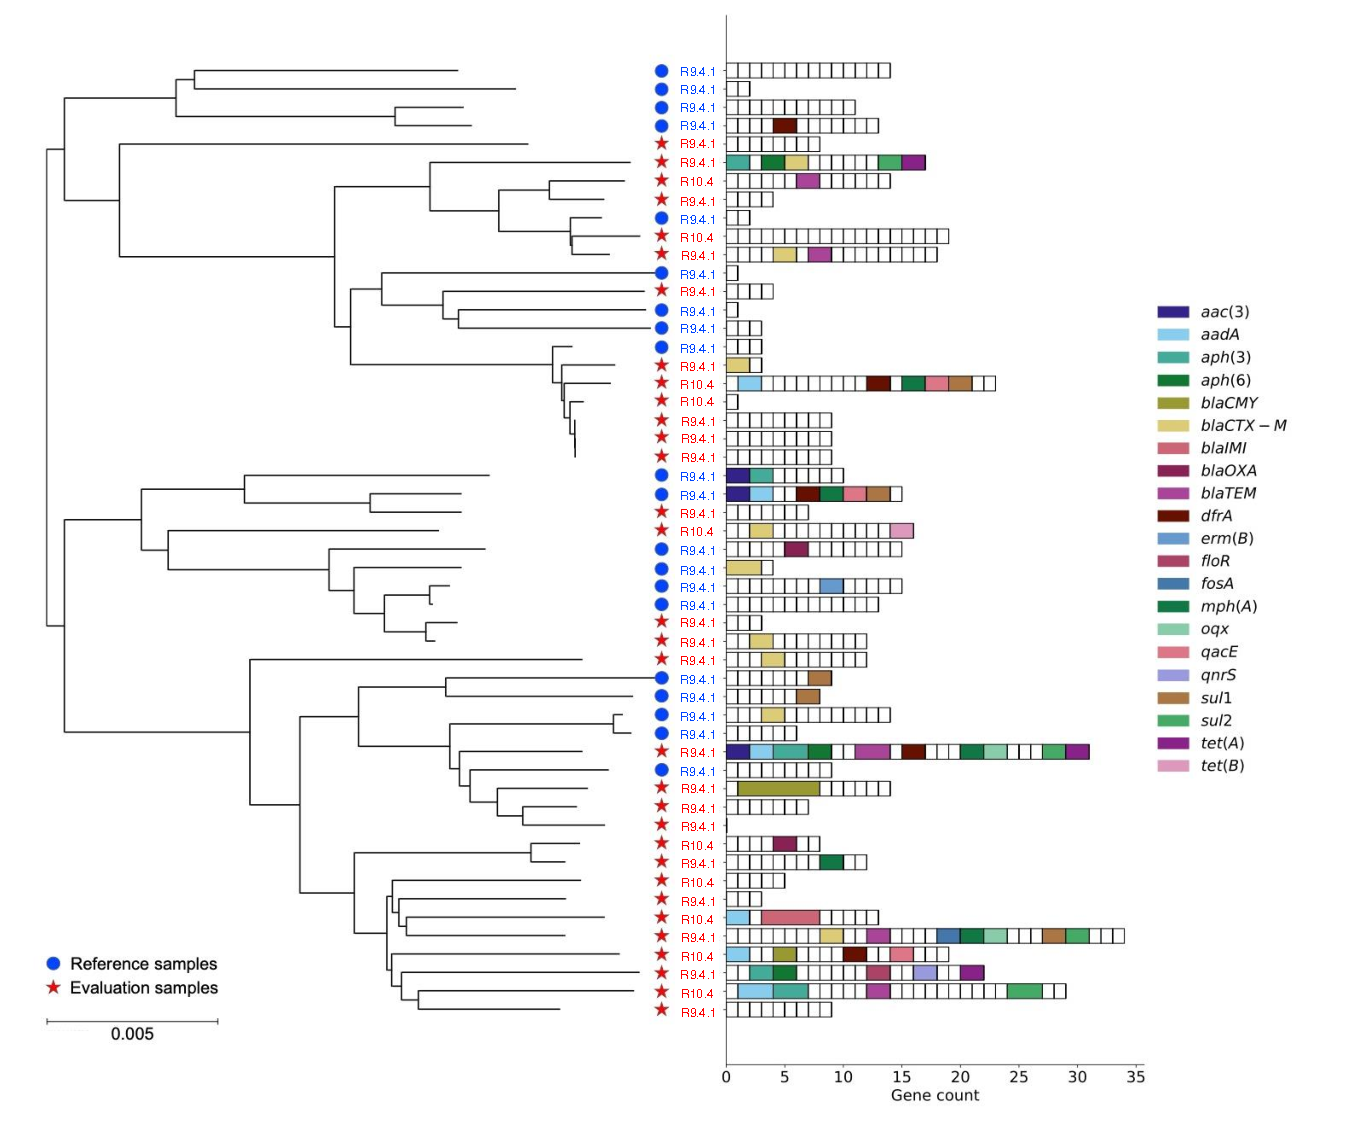
\includegraphics[width=1\linewidth]{Figures/figure_3.pdf}
\caption{A phylogeny showing the relationship between the samples used to construct the reference panRG and the samples we used to evaluate the accuracy of Amira, alongside the Nanopore flow cell and the AMR gene content of samples used in the truth evaluation. The x-axis is the number of AMR gene copies, the y-axis is the sample identifier and each block in each bar represents a unique AMR gene. AMR genes with more than one copy in a given sample have been colored. The phylogeny was constructed using mashtree v1.4.6 \cite{Katz2019} and the order of samples matches the samples at the tips in the phylogeny.}
\label{fig:3}
\end{figure*}

The mean read length across our evaluation set for the R9.4.1 samples is 14.2 kbp and Amira identified a mean of 11.9 genes per read. For the R10.4 samples, the mean read length is 4.7 kbp with 4.4 genes per read.

We compared the number and type of AMR genes found by Amira (using nanopore data) to that of AMRFinderPlus run on illumina-only assemblies generated with Shovill \cite{Shovill, Bankevich2012} (AMRFP Shovill), nanopore-only assemblies generated with Flye \cite{Kolmogorov2019} (AMRFP Flye), hybrid assemblies generated with Unicycler \cite{Wick2017} (AMRFP Unicycler), and ResFinder \cite{Bortolaia2020}. On the R9.4.1 dataset, Amira outperformed all approaches in terms of per-sample AMR gene recall, with a mean recall of 98.3\% and precision of 98.2\% (Fig.\ref{fig:4}a). In comparison, AMRFP Unicycler performed the best of the assembly methods with mean per-sample recall 97.6\% and precision 100\%. Amira also outperformed all methods on the R10.4 dataset, with a recall of 100\% and precision of 96.2\%, followed by AMRFP Flye with recall 98.1\% and precision 100\%. While we developed Amira specifically to better detect multi-copy genes, we were surprised to find that Amira excelled at detecting both single-copy and multi-copy genes in this dataset, with a mean per-gene recall of 100\% and 99.2\% respectively (Fig.\ref{fig:4}d). Amira was the only method of those tested to comprehensively identify the presence of at least one copy of each gene in the truth dataset.

The mean allelic accuracy of genes correctly called by Amira was consistently high for both the R9.4.1 and R10.4 datasets, with mean nucleotide identities of 99.8\% and 99.9\% respectively, compared to 98.4\% and 99.6\% for AMRFP Flye (Fig.\ref{suppfig:7}). On this dataset, the mean runtime of Amira was 1134 (537 - 3265) seconds with 6.5 (4.4 - 14.9) GB RAM compared to a runtime of 1856 (905 - 3939) seconds and RAM of 10.6 (9.8 - 11.4) GB for AMRFP Flye (Table.\ref{supptable:2}). 

\begin{figure*}
\centering
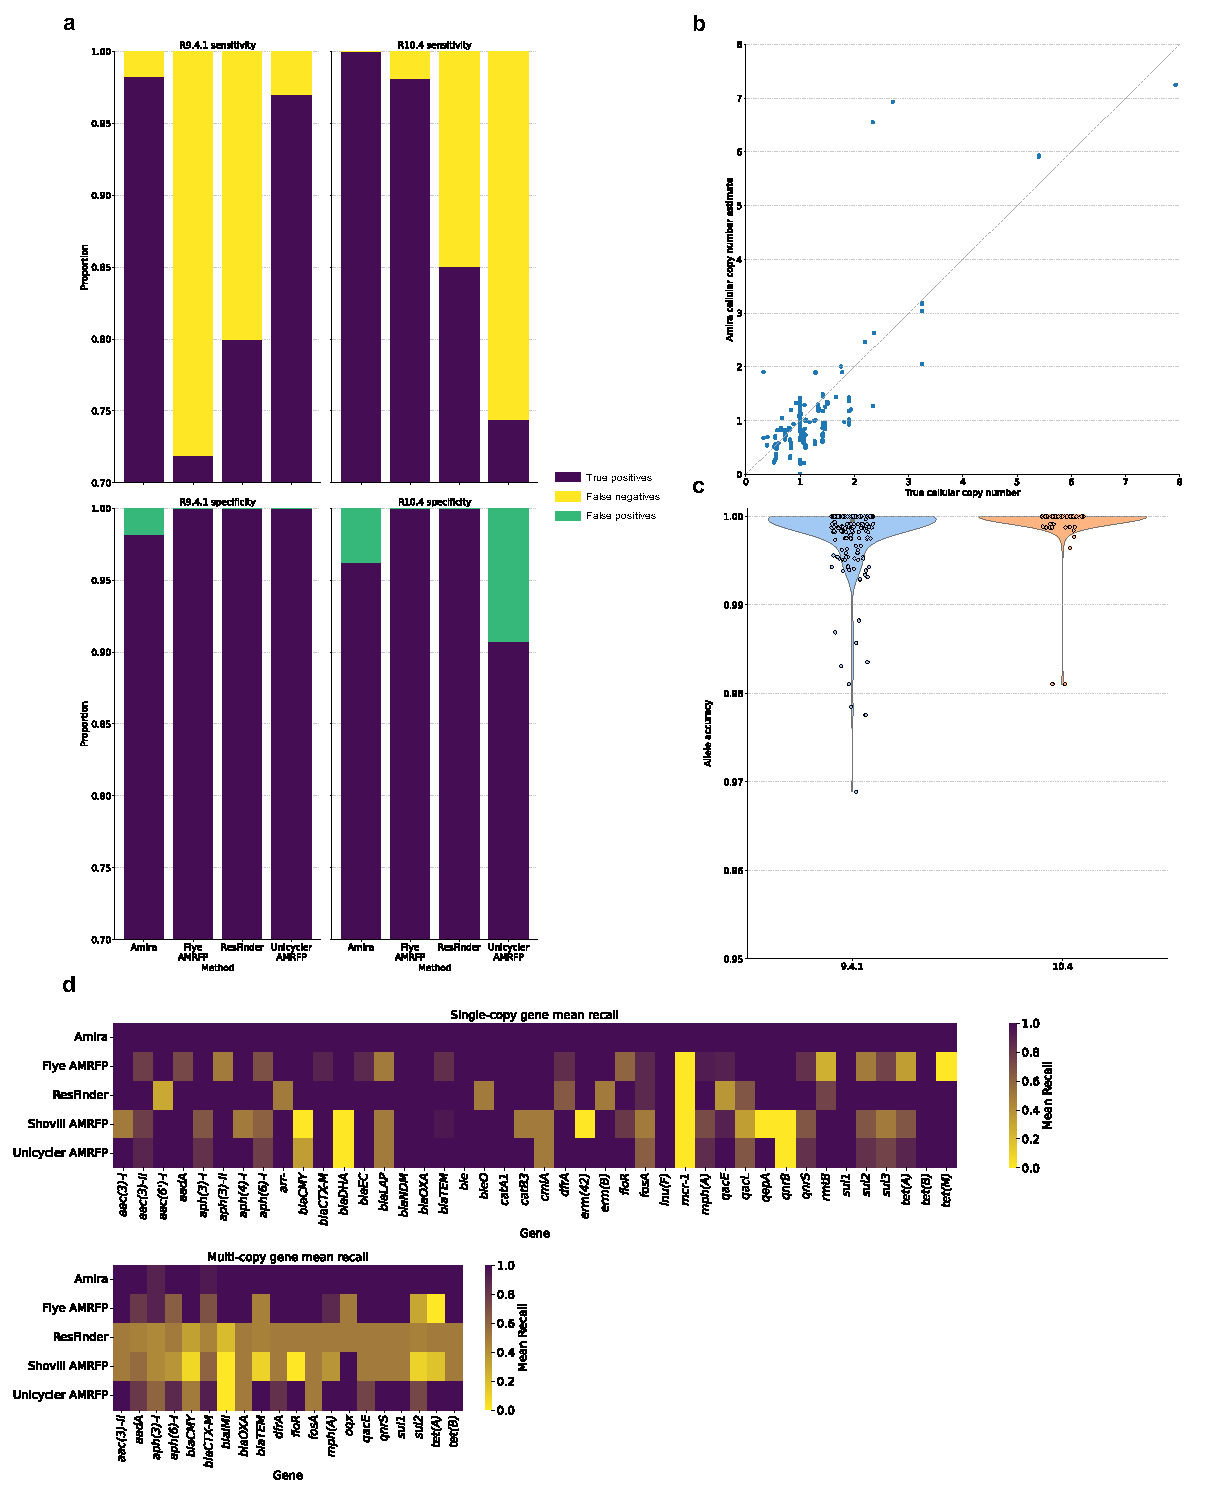
\includegraphics[width=1\linewidth]{Figures/figure_4.pdf}
\caption{(a) Sensitivity and specificity on the R9.4.1 and R10.4 samples. (b) Amira cellular copy estimates for each copy of each sample, compared to the true cellular copy number for the gene copy (estimated by dividing the mean nanopore depth across the contig by the mean depth of the longest contig). (c) Gap-inclusive nucleotide similarities between each allele output by Amira and the true nucleotide sequence. (d) Heatmaps showing the mean recall per method for each single and multi-copy AMR gene across the test samples.}
\label{fig:4}
\end{figure*}

\subsection*{Genome assembly consistently underestimates AMR gene frequencies across bacterial populations}

After finding Amira better detects single copy AMR genes than assembly-based methods, we now apply Amira with and without the optional contamination filter (Amira and Amira \texttt{–no-filtering}) to 7,830 \textit{E. coli} samples and 2,359 \textit{K. pneumoniae} with Nanopore reads available, and report the results of running AMRFinderPlus on assemblies for the same samples generated with Flye (AMRFP Flye). We report the recall of each method for detecting at least one copy of each gene in the union of all of the genes found by the three methods. On the \textit{E. coli} dataset, the mean recalls for Amira, Amira \texttt{–no-filtering} and AMRFP Flye was 53.1 (SD 44.8)\%, 98.3 (SD 12.2)\% and 31.7 (SD 35.3)\% respectively (Fig. \ref{fig:5}a). Amira also outperformed AMRFP Flye in terms of recall on the \textit{K. pneumoniae} dataset, with mean recalls of 53.4 (SD 44.8)\% and 99.4 (SD 7.6)\%, compared to 35.3 (SD 37.5)\% for AMRFP Flye (Fig. \ref{fig:5}b). For the \textit{E. coli} dataset, AMRFP identified 11\% of the genes present only in a single sample, compared to 40\% for Amira and 96\% for Amira \texttt{–no-filtering}. A similar trend held true for the \textit{K. pneumoniae} dataset, where AMRFP Flye only identified 18\% of the genes present in one sample, compared to 24\% for Amira and 97\% for Amira \texttt{–no-filtering}.

\begin{figure*}
\centering
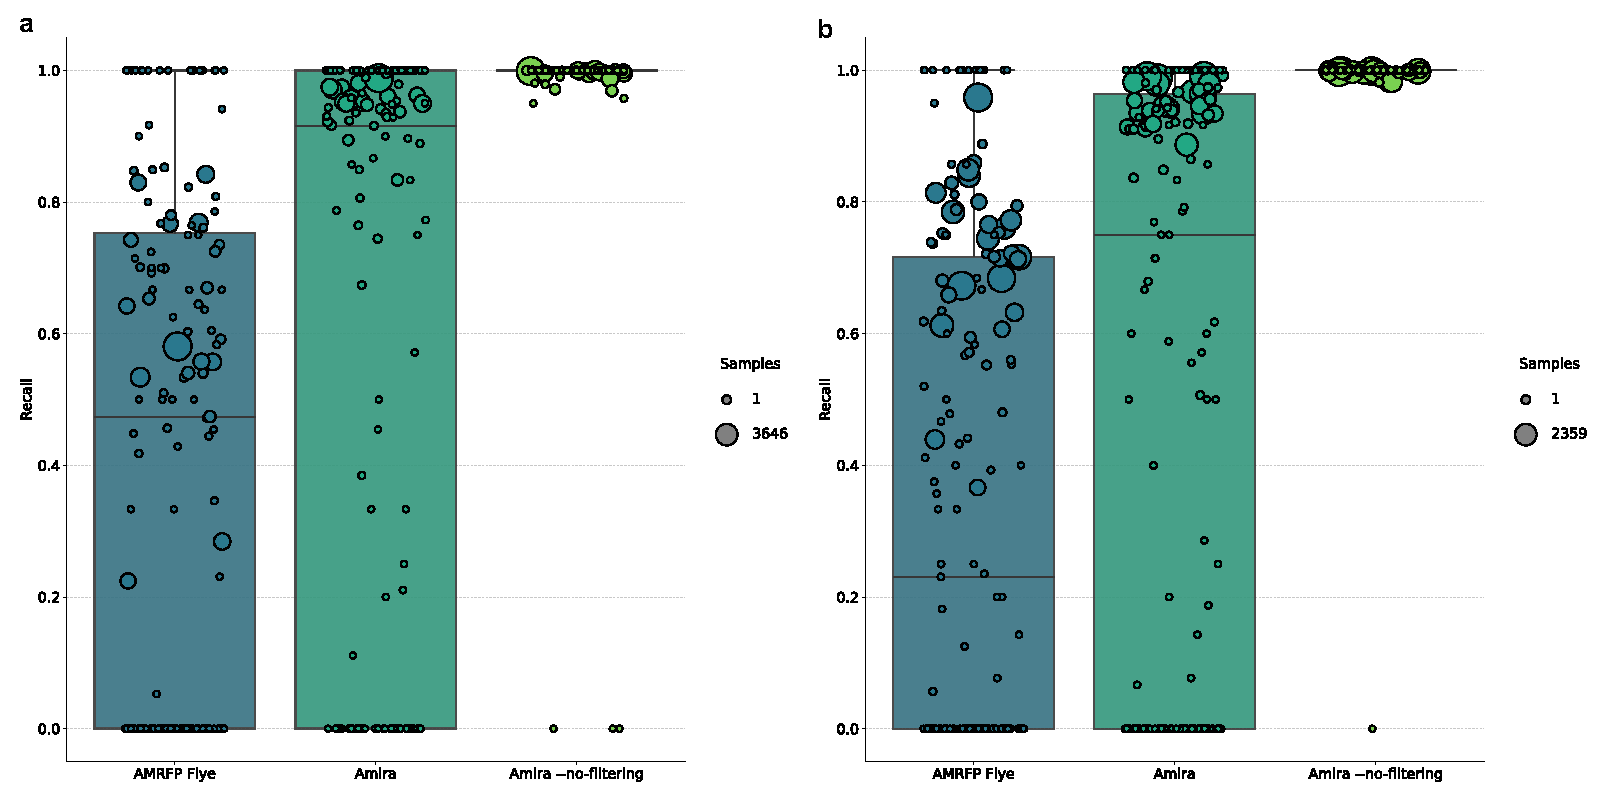
\includegraphics[width=1\linewidth]{Figures/figure_5.pdf}
\caption{Boxplots showing the per-AMR gene recall of Amira, Amira with option \texttt{--no-filtering} and AMRFinderPlus run on assemblies generated with Flye for 7,830 \textit{E. coli} (a) and 2,359 \textit{K. pneumoniae} (b) samples. Each point is a unique gene. The y-axis indicates the recall of calling at least one copy of that gene, where recall is measured as the proportion of true samples each gene is identified in, with the truth defined from the union of the three methods. Point size is scaled to the number of samples that each gene is found in.}
\label{fig:5}
\end{figure*}

\section*{Discussion}

Long read sequencing technologies, particularly using Nanopore R10.4 flow cells, have allowed significant improvements in bacterial genome assembly and the accuracy of AMR gene detection. However, genome assembly is an inherently challenging task. Bacterial genomes frequently contain duplications that can only be resolved by assemblers if sequencing reads are long enough to span the entire duplicated region. Furthermore, assembly accuracy is dependent on numerous factors that include: read depth, length and error profile, library preparation, choice of basecaller, choice of assembler and complexity of the sample under analysis \cite{FosterNyarko2023}. At present, there is no genome assembler that can produce comprehensive assemblies in every scenario \cite{10.12688/f1000research.21782.1}, which often can only be achieved through additional manual validation and correction. As genomic datasets grow larger, particularly in outbreak scenarios, the difficulty of this task increases and this highlights the need for improved methods that better leverage available sequencing technologies.

To address this challenge, we developed Amira, a tool to detect AMR genes directly from bacterial long-read sequencing data. Amira leverages the full length of long read sequences to differentiate multi-copy genes by their local genomic context. Through objective evaluation on simulated and curated truth datasets, we have demonstrated that Amira achieves substantially higher accuracy in AMR gene detection compared to existing assembly- and read-based methods. This improvement is largely driven by use of the gene as the fundamental unit. By using Pandora to identify genes on each sequencing read, Amira is robust to nucleotide-level SNP and INDEL errors, which are common in long-read sequences, as evidenced by the improvements in accuracy when retrospectively applying Amira to datasets sequenced with error-prone R9.4.1 Nanopore reads. This allows us to construct significantly cleaner graphs that more accurately capture the underlying genomic structure than conventional \textit{k}-mer based methods. 

While Amira requires prior specification of AMR genes and is not intended as a direct replacement for genome assembly, we applied it alongside several leading genome assemblers to the same long-read datasets and found consistent under-detection of AMR gene content when using assembly-based approaches. Applied to larger datasets, this leads to underestimation of gene frequencies and failure to detect rare AMR genes that may be spreading in a population. Furthermore, we have shown that the nucleotide sequences output by Amira are more accurate than those output by other long-read only approaches. While this is in part due to better differentiation of the reads containing alternate variants of the same AMR gene, it is predominantly caused by the reference-polishing approach used by Amira to obtain nucleotide sequences, whereas \textit{de novo} assembly of bacterial genomes is susceptible to false pseudogenes as a result of frameshift errors and fragmentation of open reading frames \cite{Cooley2024}. Therefore, Amira offers an accurate, automated, and user-friendly solution for AMR gene genotyping that is accessible to users without expertise in genome assembly. 

A key limitation of our approach is its reliance on read length. Unlike assembly-based methods that traverse a graph to reconstruct a genome, Amira can only differentiate the genomic contexts of AMR genes using the longest reads that cover a gene. In our tests, we had perfect recall on R10.4 Nanopore reads despite a significantly shorter read length than R9.4.1 reads, so this did not pose an issue. However, in the more complex simulated scenarios, we observe a strong positive correlation between AMR gene recall and mean read length, which can be compensated for by read depth. Read depth also plays a crucial role in nucleotide and allele calling accuracy with Amira. Genes covered by fewer reads are more likely to contain INDEL errors in the generated nucleotide sequences, and our nucleotide-space comparisons to reference alleles occasionally result in incorrect variant calls for truly present AMR genes. A future improvement could involve comparing Amira alleles in amino acid space instead. However, similar to whole genome assembly methods, this would be vulnerable to frameshift and nonsense mutation errors that can prevent the direct translation of the nucleotide sequences of identified genes.

Reference bias is a well documented challenge in bacterial genotyping methods that rely on reference sequences, which arises when a selected reference incompletely represents the diversity of a sample under analysis  \cite{pandora, 10.1016/s2666-52472100149-x, panaroo}. With Amira, we mitigate this by genotyping from a panRG constructed from a diverse set of samples that incorporates plasmid-specific genes to expand the context genes we can detect. However, as seen by the differences in AMR gene detection using Amira with and without contamination filtering, under-representation of context genes in the panRG may cause Amira to filter AMR genes from its output that are actually present in the genome of the species of interest. Therefore, it is recommended Amira is run with the contamination filtering turned off if users want to maximise sensitivity. For our purposes, there is a trade-off between panRG completeness and computational efficiency; more complete panRGs reduce the probability a truly present gene will be identified as contamination and reduce the read length requirements to differentiate AMR gene copies, but increase RAM and runtime requirements. Therefore, the gene DBGs we construct are not exhaustive and caution should be exercised when attempting to use Amira to detect multi-copy genes other than those explicitly incorporated into the panRG. 

Increasing evidence has found correlations between AMR gene dosage and MIC for specific gene-antimicrobial pairs \cite{10.1128/aac.02026-19, 10.1128/AAC.46.10.3334-3336.2002}. While MIC prediction was beyond the scope of this study, we anticipate that the more comprehensive identification of AMR gene content by Amira could enhance MIC prediction accuracy and plan to explore this in the near future. Additionally, while Amira is designed to detect AMR genes, our approach could be directly applied to estimate the genomic and cellular copy numbers of any gene of interest through minor modifications. Lastly, this work also introduces the gene DBG, a novel data structure that moves away from conventional \textit{k}-mers and is more robust to structural rearrangements that are frequent in bacteria. The gene DBG has the potential to be beneficial for a range of bioinformatic applications in place of \textit{k}-mers, particularly in bacterial genome assembly, and the approach can capture structural heterogeneity even at the level of single bacterial isolates. 

\section*{Methods}

\subsection*{Data Summary}

To construct a reference pan-genome (abbreviated to panRG) in the format required by pandora \cite{pandora}, we assembled the illumina and nanopore reads used in the 20-way analysis in \cite{pandora} with Hybracter \texttt{v0.7.3} \cite{Bouras2024} using default parameters. To supplement the panRG with plasmid-specific genes, we retrieved a FASTA of 4,056 reference alleles (as of 15 October 2024) used by MOB-suite \cite{10.1099/mgen.0.000206}. To supplement the panRG with reference sequences for acquired AMR genes, we obtained a multi-FASTA file of 7,062 (as of 21 August 2024) acquired AMR gene reference alleles
from the NCBI Bacterial Antimicrobial Resistance Reference Gene Database (Accession \textit{PRJNA313047}). 

For the simulations, we used the \textit{E. coli K-12} reference sequence (Accession \textit{NC\_000913.3}) and an \textit{ATCC 11775} reference plasmid (Accession \textit{CP033091.2}) as the backbone for our simulated assemblies. To evaluate Amira on truth data, we retrieved the RefSeq assemblies and the illumina and nanopore reads for 32 \textit{E.coli} isolates in table \ref{supptable:1}. Ten of our samples were sequenced using R10.4 flow cells (referred to as the R10.4 samples) and 22 using R9.4.1 flow cells (referred to as the R9.4.1 samples).

\subsection*{Obtaining truth assemblies}

We retrieved the illumina and nanopore reads for 32 \textit{E.coli} isolates in supplementary table xxxx, as well as the RefSeq assemblies for the 22 samples sequenced using R9.4.1 Nanopore reads. For the ten R10.4 samples, Trycycler v…. Was used to generate consensus assemblies from individual assemblies using Flye? V…, Unicycler? V… hybrid and …. We mapped the illumina and nanopore reads to the Trycycler and RefSeq assemblies using minimap2 \texttt{v2.28} \cite{10.1093/bioinformatics/bty191} with options \texttt{--eqx -a -x sr --secondary=no} for the illumina reads, and \texttt{--eqx -a -x map-ont --secondary=no} for the nanopore reads. We visualised the nanopore read depths across each assembly, normalised by the mean read depth for each contig containing an AMR gene, to check for regions of elevated coverage that may indicate collapsed duplications. We identified the presence of collapsed duplications in two samples. We subsetted the reads mapping to the problematic contigs with samtools \texttt{v1.17} \cite{Li2009} and pyfastaq \texttt{v3.17.0} and reassembled the long reads mapping to the problematic contigs using Canu v2.3 \cite{Koren2017} with \texttt{genomeSize=20k}, then conducted one round of short-read polishing with polypolish v0.6.0 \cite{10.1099/mgen.0.001254}. We used TNA \texttt{v0.3.0} \cite{TNA} to visualise the alignments of the reassembled contigs to the reference. Some plasmids may be missing from Nanopore only/first assemblies depending on the library preparation technique used prior to sequencing. Therefore, we assembled the illumina reads for each sample with Shovill \texttt{v1.1.0} and supplemented the reference assemblies with any contigs that contained unique AMR genes not already present in the reference assemblies. Further information detailing the assembly validation be found in figures \ref{suppfig:1}-\ref{suppfig:6}.

\subsection*{Constructing species-specific panRGs}

Amira relies on Pandora \cite{pandora} to obtain an ordered list of genes and gene directions on each sequencing read. We developed a snakemake \cite{10.1093/bioinformatics/bts480} workflow to automate the construction of Pandora panRGs from a set of reference assemblies that we then supplement with a multi-FASTA file of acquired AMR and plasmid-specific reference genes. This begins by annotating the genes in a set of reference assemblies using bakta \texttt{v1.7.0} \cite{Schwengers2021}, then clusters the annotations into orthologs using Panaroo \texttt{v1.5.0} \cite{panaroo}  with \texttt{--clean-mode sensitive --refind-mode off --remove-invalid-genes --length\_outlier\_support\_proportion 0.1 --merge\_paralogs --threshold 0.8 and --len\_dif\_percent 0.0}. We then filter all alleles less than 250 bp in length and all transposase or IS-related genes, as these are frequently fragmented in bacterial genomes and a significant source of inconsistent gene calls. After aligning the filtered clusters, we then run make\_prg \texttt{v0.5.0} with default parameters, and construct a panRG using Pandora \cite{pandora} index \texttt{v0.12.0}, specifying \texttt{-k 15 -w 5}. 

\subsection*{Constructing a read-coherent de Bruijn graph in gene space}

Amira takes a pseudo-SAM file that is output by Pandora and specifies the genes identified on each read and from this, creates a dictionary where the keys are read identifiers and values are an ordered list of gene identifiers, where the orientation of each gene relative to the sequence of the gene in the panRG is the prefix of each gene identifier. We construct a \textit{de Bruijn} graph in gene space (gene DBG) using the gene calls for each read. For all reads with at least $k$ genes, we slide a window of size $k$ across the list of genes to obtain $n - k + 1$ “gene-mers”, analogous to \textit{k}-mers used in sequence assembly. We iterate through each gene-mer in a read, and add a node to the graph by populating a hash table, with the key being the hash value of the canonical gene-mer. For each pair of adjacent gene-mers we also create two edges, with one edge storing the direction of the target gene-mer relative to the canonical of the source gene-mer, and one edge the direction of the source gene-mer relative to the canonical target gene-mer.

\subsection*{Correcting false paths in the graph}

We found that transposases and IS-related genes were commonly present in \textit{E. coli} genomes in fragmented form, making it difficult for Pandora to decide whether a fragment of a gene was simply a random repeated sequence that should be ignored or a genuinely present gene. However, we aim to detect full-length genes to construct gene DBGs and chose to exclude these from the panRG to remove most systematic errors. Amira uses several methods to account for the remaining errors caused by false negative and positive gene calls, first applying correction to the graph itself, then using the corrected graph to correct the underlying list of genes on each sequencing read.  

After constructing the initial graph and discarding all nodes that do not contain any reads with an AMR gene, we filter out reads where >80\% of the nodes have a depth of one. After rebuilding the graph, we apply an iterative correction algorithm that consists of two stages: dead end removal and path replacement. The dead end removal stage finds and removes all paths that start at a node with an in degree or an out degree of zero, end at a node with a degree greater than two and contain fewer than $k$ nodes in its path.
 
Path replacement begins by conducting a depth-first-search between all combinations of pairs of nodes with an in or out degree greater than one, to obtain an aggregated list of all of paths that are less than or equal to three times $k$ nodes in length. We then filter out all paths that are wholly contained within another path, and sort the remaining paths from longest to shortest. The sorted paths are clustered together based on their start and end nodes and we iterate through the clusters from longest maximum length to shortest and sort the paths in each cluster from highest mean coverage to lowest. We then iterate through all paths in the sorted cluster with index $i$ and for each iterate through all lower coverage paths with index $j$ where $j > i$. We use sourmash \texttt{v4.8.4} \cite{Pierce2019} to extract the minimizers from the reads causing each path in a pair, specifying a \textit{k}-mer size of 13 and scaled parameter of 10 and correct the reads following a low coverage path to follow a high coverage path if $\ge$80\% of the minimizers in one of the paths is contained within the other.

\subsection*{Assigning reads to paths}

For each copy of each AMR gene in a bacterial sample, there exists a minimum length path through the corrected gene DBG that incorporates a sufficient number of context genes to make it distinct. When the genomic context immediately flanking each copy of a multi-copy AMR gene differs, only one context gene is needed. However, in cases where the number of genes within a duplicated genomic region significantly exceeds the value of $k$, it is necessary to leverage the full read length to differentiate the paths. 

We address this by first identifying blocks of contiguous nodes that contain AMR genes that are observed in the reads (Fig.\ref{fig:6}a). This enables differentiation of the reads that contain multi-copy genes but with a different immediate genomic context within $(k - 1) / 2$ genes upstream or downstream of an AMR gene, or a tandem array of duplicated genes. To achieve this, we construct a generalised suffix tree, where each "letter" represents a node identifier, and each "word" corresponds to the ordered list of node identifiers on a read. Each read contributes two words to the suffix tree: one representing the forward list of nodes and the other for its reverse. We refer to this as the primary suffix tree. For each unique AMR gene, we then identify the set of “anchor” nodes, which are nodes that contain the AMR gene and are adjacent to nodes not containing the AMR gene in any read. For every anchor node, we extract all downstream sub-lists of nodes using the primary suffix tree and construct a secondary suffix tree from the reverse of the suffixes that contain the anchor node. By searching within this secondary suffix tree, we efficiently identify all paths between pairs of anchor nodes and determine their frequencies. We will refer to these as internal blocks (Fig.\ref{fig:6}b).

After identifying all internal blocks, we then look at the paths of nodes external to each block to differentiate long duplicated regions where the paths diverge outside of the internal block. This is achieved by querying the primary suffix tree for each internal block, tracking the suffixes and storing them as downstream external blocks. Simultaneously, we query the reverse of the block and store the reverse suffixes as upstream external blocks. We separately cluster the upstream and downstream external blocks for each internal block if they are sub-paths of a longer clustered external block, ignoring all paths that are sub-paths of the paths in more than one cluster. Subsequently, we choose the shortest path in each cluster as the representative for the external block, and join the upstream external block, internal block, and downstream external block that share at least one read and filter out any paths that are sub-paths of longer paths (Fig.\ref{fig:6}c). We then attempt to minimize the number of context genes necessary to differentiate the paths by converting each node-space path into gene space and get all possible sub-paths that are not sub-paths of any other full-length path and still contain the same number of copies of the AMR gene as the full-length path. We finally select the sub-path that is covered by the most reads as the minimum-length final path (Fig.\ref{fig:6}d). 

We collect all reads containing each final path and store the nucleotide sequences for each AMR gene copy at index $g$ in the path and estimate the copy number of each AMR gene copy to account for multi-copy plasmids with identical AMR gene content. We do this by estimating the mean read depth across the longest read containing each AMR gene copy, and normalise it by the mean read depth across core genes that have been identified by Pandora.

\begin{figure*}
\centering
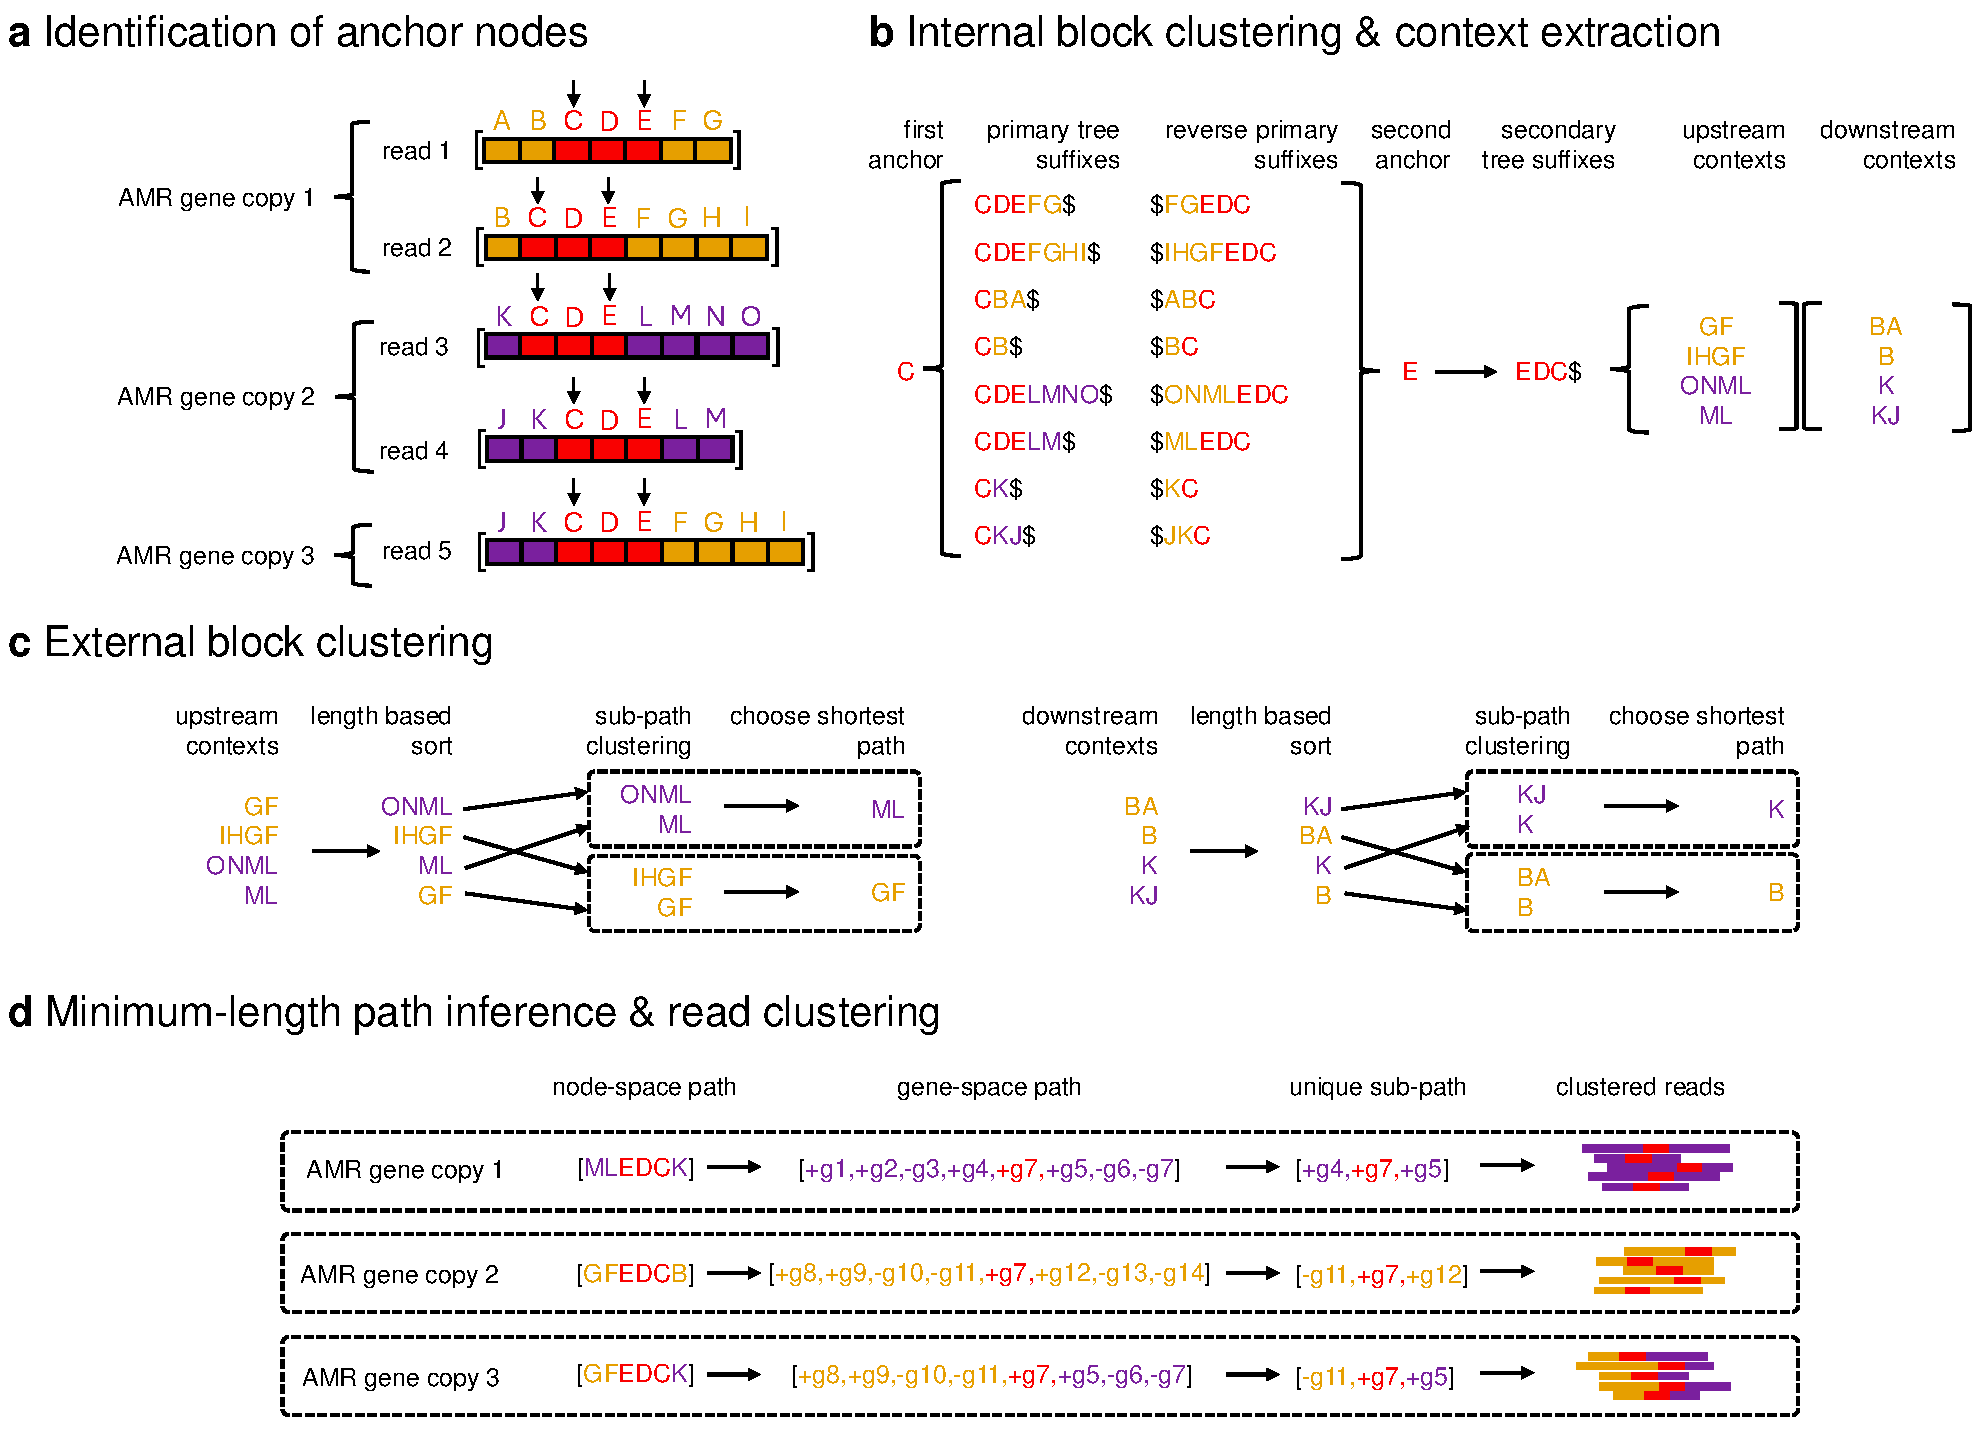
\includegraphics[width=1\linewidth]{Figures/figure_6.pdf}
\caption{The approach used by Amira to separate the reads containing multi-copy AMR genes using paths through the corrected gene DBG. (a) The set of “anchor” nodes are identified for each unique AMR gene. These are nodes containing the AMR gene that occur immediately adjacent to any node not containing the AMR gene in any read. (b) Internal blocks are defined between pairs of anchor nodes. This process begins by identifying the suffixes of the first anchor by querying a suffix tree built from the list of node identifiers for each read. Next, the second anchor node is queried in a second suffix tree constructed from the reverse of the suffixes obtained in the initial search. The blocks of nodes external to each internal block are then obtained. (c) External blocks are clustered into underlying paths. Blocks are sorted from longest to shortest, and clustered with a longer block if they are entirely contained within it. Blocks that belong to multiple clusters are disregarded and the shortest block within each cluster is selected as the representative. (d) Minimum-length paths that differentiate AMR gene copies are inferred and reads are clustered by the presence of these paths. Full-length paths in node space are determined by joining external and internal blocks that share at least one read, then converted to gene-space paths. For each gene-space path, all sub-paths are enumerated and the single sub-path that is not a sub-path of any other gene-space path, contains the same number of AMR genes as the full length path and is covered by the most reads is chosen as the minimum-length path. Reads are clustered based on the presence of the minimum-length paths.}
\label{fig:6}
\end{figure*}

\subsection*{Obtaining AMR gene alleles}

The final step is to obtain the allelic sequences of each AMR gene copy. We take the clusters of nucleotide sequences defined previously, then create a FASTQ file of these sequences and use minimap2 \texttt{v2.17} \cite{10.1093/bioinformatics/bty191} to map the reads to all reference alleles that are contained in the cluster of orthologous genes of that AMR gene. We choose the reference allele that most closely matches the reads with identity $\ge$90\% and coverage $\ge$90\% by default, and conduct five iterations of polishing using racon \texttt{v1.5.0} \cite{10.1101/gr.214270.116} to obtain the final sequence of each AMR gene copy. We apply an optional contamination filter to the final Amira output that removes all AMR gene copies where none of the reads assigned to the gene contain any non-AMR context genes.

\subsection*{Evaluating on simulated data}

We developed a snakemake \cite{10.1093/bioinformatics/bts480} workflow to simulate \textit{E. coli} samples with varying complexities in AMR gene content to assess the accuracy of Amira gene calling and its correlation with read depth and length. We used the \textit{E. coli K-12} reference chromosome and removed the sequence of a single copy of \textit{blaEC} at positions 4377811-4378944 to act as the backbone of a simulated chromosome, and an \textit{ATCC 11775} reference plasmid that contains no AMR genes. Our workflow spikes in complex AMR regions identified from the literature, then simulates sequencing read sets for input into Amira using badread \texttt{v0.4.1} \cite{Wick2019}, using \texttt{--error\_model "nanopore2023"} and all combinations of parameters: \texttt{--quantity “10x”, “20x”, “40x”, “80x”} and \texttt{--length “5000,6615.5”, "10000,10815.5", "20000,19215.5", "40000,36015.5"}. We simulated reads using just the backbone chromosome and plasmid as a negative control, then simulated five additional test cases identified from public datasets. We then compared the AMR gene recall of Amira \texttt{v0.6.4} to Flye \texttt{v2.9.3} with AMRFinderPlus \texttt{v3.12.8} \cite{Feldgarden2021} with database \texttt{v2024-01-31.1} and options \texttt{--plus --organism Escherichia}. Genes with “PARTIALX” or “PARTIALP” in the “Method” column of the AMRFinderPlus output were excluded.

\subsection*{Evaluating on real data}

We defined the true AMR genes in our test set as any sequence within our test assemblies that is at least 90\% identical and 95\% covered by a reference allele included in the panRG. We did this by mapping all AMR gene reference alleles included in the reference panRG using minimap2. We filtered all hits with alignment coverage <95\% and identity <90\% and sorted all remaining hits first by identity, then by length, choosing the best match in cases where multiple alleles overlapped with each other. False pseudogenes are frequent in bacterial assemblies and this relaxed coverage threshold avoids penalisation of AMR genes that are present in the samples but where base-level errors cause frameshifts or premature stop codons within open reading frames. All of the tools tested call AMR genes that are less than 100\% covered by a reference. 

We subsampled the nanopore read sets for each sample to 200x using rasusa \texttt{v2.1.0} \cite{Hall2022}  and compared the accuracy of Amira \texttt{v0.6.4} to that of AMRFinderPlus \texttt{v3.12.8} \cite{Feldgarden2021}, with database \texttt{v2024-01-31.1} and options \texttt{--plus --organism Escherichia}, run on illumina-only assemblies generated with Shovill \texttt{v1.1.0} \cite{Shovill, Bankevich2012}, nanopore-only assemblies generated with Flye \texttt{v2.9.3} \cite{Kolmogorov2019} and hybrid assemblies generated with Unicycler \texttt{v0.5.0} \cite{Wick2017}. All assemblers were run using their default parameters and genes with “PARTIALX” or “PARTIALP” in the “Method” column of the AMRFinderPlus output were excluded. We also ran Resfinder \cite{Bortolaia2020} \texttt{v4.6.0} on the nanopore reads for each sample with options \texttt{-s e.coli -acq --nanopore} by generating an index of all AMR alleles in our reference panRG using kma\_index \texttt{v1.4.15} \cite{Clausen2018}. We excluded all ResFinder hits with <90\% identity or <90\% coverage. The cellular copy numbers of each AMR gene were estimated by obtaining the mean nanopore read depth across the contig for the gene, then normalising by the mean read depth across the longest contig in each sample. All alleles for each unique AMR gene present in both the reference assembly and the output of the evaluated tool were aligned using MAFFT \texttt{v7.526} \cite{mafft} and option \texttt{–auto}. Nucleotide-level accuracies were then calculated as the proportion of matching columns in the alignment between each reference allele and the output allele. Each output allele was then matched to the closest reference allele without replacement, prioritising nucleotide accuracy and then absolute difference in cellular copy number. 

We found that diverging paths in a single connected component of the Amira graph were resulting in false positive gene calls in one sample. By subsetting the reads unique to the differing paths and visualising the pileups with IGV \texttt{v2.19.1} \cite{10.1093/bib/bbs017}, we found this was the result of the presence of a minor frequency structural variants of a plasmid in this sample (Fig.\ref{suppfig:8}). We chose not to penalise the assemblers for missing the low-frequency variant, nor penalise Amira for identifying it as it resulted from genuine heterogeneity present in the read sets.

\subsection*{Running Amira on large nanopore datasets}

Following evaluation of Amira on simulated scenarios and a curated truth dataset, we next use Amira to retrospectively analyse all \textit{E. coli} and \textit{K. pneumoniae} samples in the ENA with long reads available (as of 11th February 2025). Using the ENA browser, we obtained a TSV of all run accessions for Tax Id 562 for \textit{E. coli}, and Tax Id 563 for \textit{K. pneumoniae}, and downloaded all read sets containing the terms “Nanopore”, “MinION”, “PromethION” or “PacBio” in the “description’ column of the TSV. We then ran Amira \textit{v0.6.4} with default parameters, Amira with option \texttt{–no-filtering} and AMRFinderPlus \texttt{v3.12.8} with options \texttt{–plus –organism Escherichia} or \texttt{Klebsiella\_pneumoniae} on nanopore-only assemblies generated with Flye \texttt{v2.9.3} with default parameters. We defined the true AMR genes present in each sample as the union of the unique genes called by all methods, then calculated the recall of each method for reporting the presence of each gene across the dataset. We excluded samples that failed to assemble with Flye and genes with a value of <90\% in the “\% Coverage of reference sequence” column of the AMRFinderPlus output.

\subsection*{Data and code availability}

Amira is freely available from \url{https://github.com/Danderson123/Amira} under an Apache-2.0 license and installable via PyPI. The panRG construction pipeline is available from \url{https://github.com/Danderson123/Amira_panRG_pipeline}. The scripts to recreate the figures in this paper are available at \url{https://github.com/Danderson123/amira_paper}. The \textit{E. coli} panRG is available from \url{https://drive.google.com/file/d/13c_bUXnBEs9iEPPobou7-xEgkz_t08YP/view?usp=sharing}, the \textit{K. pneumoniae} panRG is available from \url{https://drive.google.com/file/d/1DYG3QW3nrQfSckIX9Vjbhbqz5bRd9W3j/view?usp=drive_link} and the \textit{E. faecium} panRG is available from \url{https://drive.google.com/file/d/1AzzFNRbH6VXPj5CX2txlcxhW8AhL9HSh/view?usp=sharing}. The accessions for the long reads, short reads and reference assemblies for all evaluation samples are available via figshare and can be found in table \ref{supptable:1}.

\section*{Acknowledgements}
The authors are very grateful to Martin Hunt for advice on fixing assemblies, William Matlock for guidance on MIC prediction, and John Lees, Julian Parkhill and Nassos Typas for their valuable advice, guidance and support throughout the project as part of the thesis advisory committee for DA. We also thank Wei Shen and Daria Frolova for their general interest and providing fruitful discussion during the undertaking of this work.

\section*{Contributions}
Conceptualization: D.A., Z.I. Data Curation: D.A, T.L., R.W., L.J. Formal analysis: D.A. Funding acquisition: J.L., Z.I. Investigation: D.A. Methodology: D.A., L.L, Z.I. Project administration: Z.I. Resources: R.W., L.J., Z.I. Software: D.A. Supervision: Z.I. Validation: D.A. Visualisation: D.A. Writing – original draft: D.A., R.W., Z.I. Writing – review \& editing: D.A., Z.I.

\section*{Bibliography}
\bibliographystyle{bxv_abbrvnat}
\bibliography{refs.bib}